\chapter{Fetch Stage}

We are ready to build our fetch stage.  To do this, we will make one more module, our instruction memory.  Then we will make a module to assemble all of our modules together into a working fetch stage.


\section{Instruction Memory Module}
Instructions are stored in memory and are accessed by using the address where they are stored.  You can think of memory like a giant hotel for our data.  Each piece of data is stored in a room (memory location), which we can find by its room number (memory address).  To get a piece of data stored in memory (like an instruction) we need to take its address, go to that location, and grab the data.  In Verilog, a bunch of memory locations that are accessed by an address is called an array.  Arrays in Verilog are declared like they are in C; the data type is specified, then the name, then the array size.  

To store the instructions, we will need an array of 32-bit numbers (definitions.vh defines INSTR\_LEN as 32, please use this macro), which means the data type must be \verb2reg[`INSTR_LEN-1:0]2.  After the name is specified (imem in this case), we are going to use a parameter called SIZE to specify how many elements the array has: \verb2[SIZE-1:0]2.  Therefore, your array will be defined as \verb2reg[`INSTR_LEN-1:0] imem [SIZE-1:0]2.

Now we need to populate this array with instructions.  Rather than populating the array element by element, we will read the instruction values in from a file called instrData.data that I have provided in the testfiles area of the ARM-Lab repository.  Note that we are just initializing the array with the values from the file.  The values should only be read from the file once at the beginning of the simulation.  Then we will access the imem array for an instruction value. To read the file and put the contents into our imem array, we will use \$readmemh to read in hexadecimal values from instrData.data.  \$readmemb could be used if we chose to format our data file in binary rather than hexadecimal.  It is very important that we use a macro in definitions.vh for the name and path of the instrData.data file, as this might change and it will be necessary for grading.  Make sure to update the definition of IMEMFILE to point to your ARM-Lab/testfiles directory (as opposed to the potter/ARM-Lab/testfiles directory).  The line of code to read the data in from the file is \verb2$readmemh(`IMEMFILE, imem);2

Once the array is populated, we can access imem and provide the instruction that corresponds to the requested address.  Instructions should only be updated on the positive edge of the clock.  I have provided a complete testbench for this module.  I have also provided a partially complete file called instr\_mem.v in code/1\_fetch directory.  Complete the module code to make a working instruction memory module.  Test it against instr\_mem\_test.sv and verify that the module works as expected.  The test will compare your instruction output to the instruction values that I provided in instrData.data. 

\section{Fetch Stage}
Now we need to connect our modules together to make a fetch stage.  The components of our instruction fetch (sometimes called ifetch or just fetch) stage are shown in Figure~\ref{fig:fetch}.

\begin{wrapfigure}{L}{2in}
\caption{Instruction Fetch Stage.}\label{fig:fetch}
\begin{center}
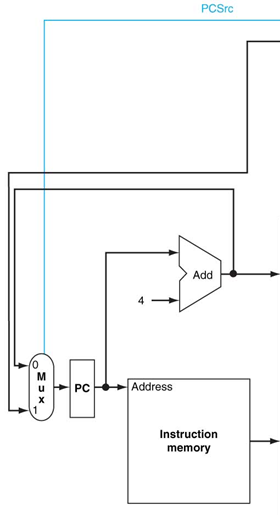
\includegraphics[width=2in]{../images/pipeline_fetch.png}
\end{center}
\end{wrapfigure}

Any wire (or reg) that comes into or goes out of the figure are input or output ports of the iFetch module.  In Figure~\ref{fig:fetch}, the blue wire is a control signal and comes ultimately from the control unit, which you will build in the decode stage.   Wires (or regs) that are completely contained in the figure are local to the iFetch module and are thus defined internally in the module (not an input or output).  The one exception to this is the current program counter (cur\_pc).  While there is no reason (at this point) that it must be output from the iFetch module, you must still make it an output so that it shows up on your simulation results, helping you to keep track of the program counter for the instruction that is currently executing.  And it is required to verify functionality with the testbench.

While the input and output signals are easily identified by the diagram, you must also determine the size of each signal and whether it is a wire or reg.  When you look at the figure I cut from a figure in the book, note that I labeled every wire on the diagram in green.  For the sake of consistency and debugging, it is required that you use these names.  

IMPORTANT NOTE: Throughout your entire project, your signal names should follow the convention of the Freescale Semiconductor Verilog guide, which states that signal names should be all lower case, with words separated by an underscore.   

Once you have figured out all your connecting signals (wires and regs), you should identify the components you are going to use.  We have already created the modules, so now we just need to tell Verilog to instantiate them in the iFetch module and connect them together.  Create the iFetch module in a new file called iFetch.v in the code/1\_fetch directory.  

I have provided a complete testbench called iFetch\_test.sv.  Use this testbench to determine if your fetch stage is working properly.  As we progress through this lab project, you will learn how critical timing is.  Please look at the cur\_pc value and the instruction value and verify that the instruction that was fetched is the correct instruction, according to instrData.data and the current program counter.  Note that no instruction should be fetched in the first 5ns, as this is a half clock cycle and does not have a rising edge.  

I have included a file called delay.v in code/0\_common.  It includes a module that inputs a clock signal and outputs a clock signal that is delayed by some number of ns.  This will be useful when resolving timing issues.  Throughout this entire lab project, the delay module should only be instantiated in the top-level module (testbench).  If you need the output of the delay function in a lower-level module, add a port to the lower-level module and pass it through that port.


\section{Your Assignment}
You are to:
\begin{enumerate}
\item Complete the instruction memory module.
\item Verify the module by running against the provided testbench.
\item Create the iFetch stage.
\item Verify the module by running against the provided testbench.
\item Produce a landscape mode PDF called Lab3\_lastname.pdf that includes (in this order):
\begin{enumerate}
\item Your name and the lab number.
\item A snip of the Simulation Results for the instr\_mem\_test.  Please show all values in decimal except for the instructions.  Please show instructions in hex.
\item The instr\_mem\_test results copied and pasted from the Tcl Console.  The results should show the entire log from BEGIN TEST RESULTS to END TEST RESULTS.
\item A snip of the Simulation Results for the iFetch\_test.  Please show all values in decimal except for the instructions.  Please show instructions in hex.  
\item The iFetch\_test results copied and pasted from the Tcl Console.  The results should show the entire log from BEGIN TEST RESULTS to END TEST RESULTS.
\end{enumerate}
\item Upload Lab3\_lastname.pdf file to Canvas.
\item Zip up your ARM-Lab directory and submit it on Canvas as well.  Please make sure that you give me the ARM-Lab directory rather than the ARM-Project directory.  I do not want the project files in the ARM-Project directory.  Before you submit your zip file, extract the file and make sure that the top-level directory is called ARM-Lab and that the lower level directories like code, manual, etc are directly beneath ARM-Lab in the directory structure.  I will extract your zip file and run your code against my correct testbench to verify that your code and testbench work correctly, and it is critical that everyone's directory structure is consistent.
\end{enumerate} 